\section{Introduction}
How did the Sun form, how the Earth? To answer such fundamental questions, we cannot travel back in time, but we can study objects that are very similar to our Sun's progenitor: Young stellar objects that will evolve into a stellar system like ours. In this review, we concentrate on stellar systems broadly resembling the young Sun's, i.e., with stellar masses below about 2$\,M_\odot$.

Most, if not all, stars and planets form in molecular clouds, often associated with cool and dense filaments that collapse into proto-stars. In these regions, gravity dominates over the stabilizing effects of thermal pressure, turbulence, and magnetic fields \citep[e.g., ][]{McKee_2007} and protostars form  \citep{Andre_2014}. The first self-gravitating and hydrostatic core contains only a small fraction of the final stellar mass ($\sim0.01\,M_\odot$). At this time most of the mass is still in an extended envelope \citep[e.g.,][]{Gong_2015,Lee_2020}. These early objects are called class~0 \citep[see Fig.~\ref{fig:starform_classes} top left, and ][]{Andre_1993, Larson_2003}. Due to angular momentum conservation, a disk forms around the central condensation and outflows are launched, which regulate the angular momentum balance of the system. Collimated jets propagate into the interstellar medium beyond the envelope and are often the first detectable signs of a forming star. In this phase, accretion proceeds through the disk onto the protostar while the material from the envelope replenishes the disk \citep{Padoan_2014}, which itself contains only a small fraction of the stellar mass ($\sim0.01\,M_\odot$). After roughly $10^5$\,yrs the protostar's mass rivals the envelope (class~{\sc i}, Fig.~\ref{fig:starform_classes} top right). The central object is hotter and more luminous than class~0 objects, and planets can form around them.

Eventually, the envelope disperses and the central star becomes visible at optical wavelengths at a stellar age of $\sim1\,$Myr; at this stage, they are called class~{\sc ii} objects or classical T Tauri stars (CTTS). The envelope dispersal mechanism is not clear yet, but winds and radiation from any nearby OB stars or otherwise radiation and outflows from low mass stars likely play a major role. Also, the winds launched by the forming stellar system itself may contribute to the envelope dispersal and reduce the envelope-to-stellar-mass conversion efficiency \citep{Frank_2014}. Accretion proceeds and begins to reduce the disk mass, while planet formation continues. In this stage,  we often get a first relatively unobscured view to the newborn stars (Fig.~\ref{fig:starform_classes} bottom left). In summary, ``The fundamental problem of star formation is how stars [get] their mass'' \citep{Dunham_2014}.


\begin{figure}[t]
\centering
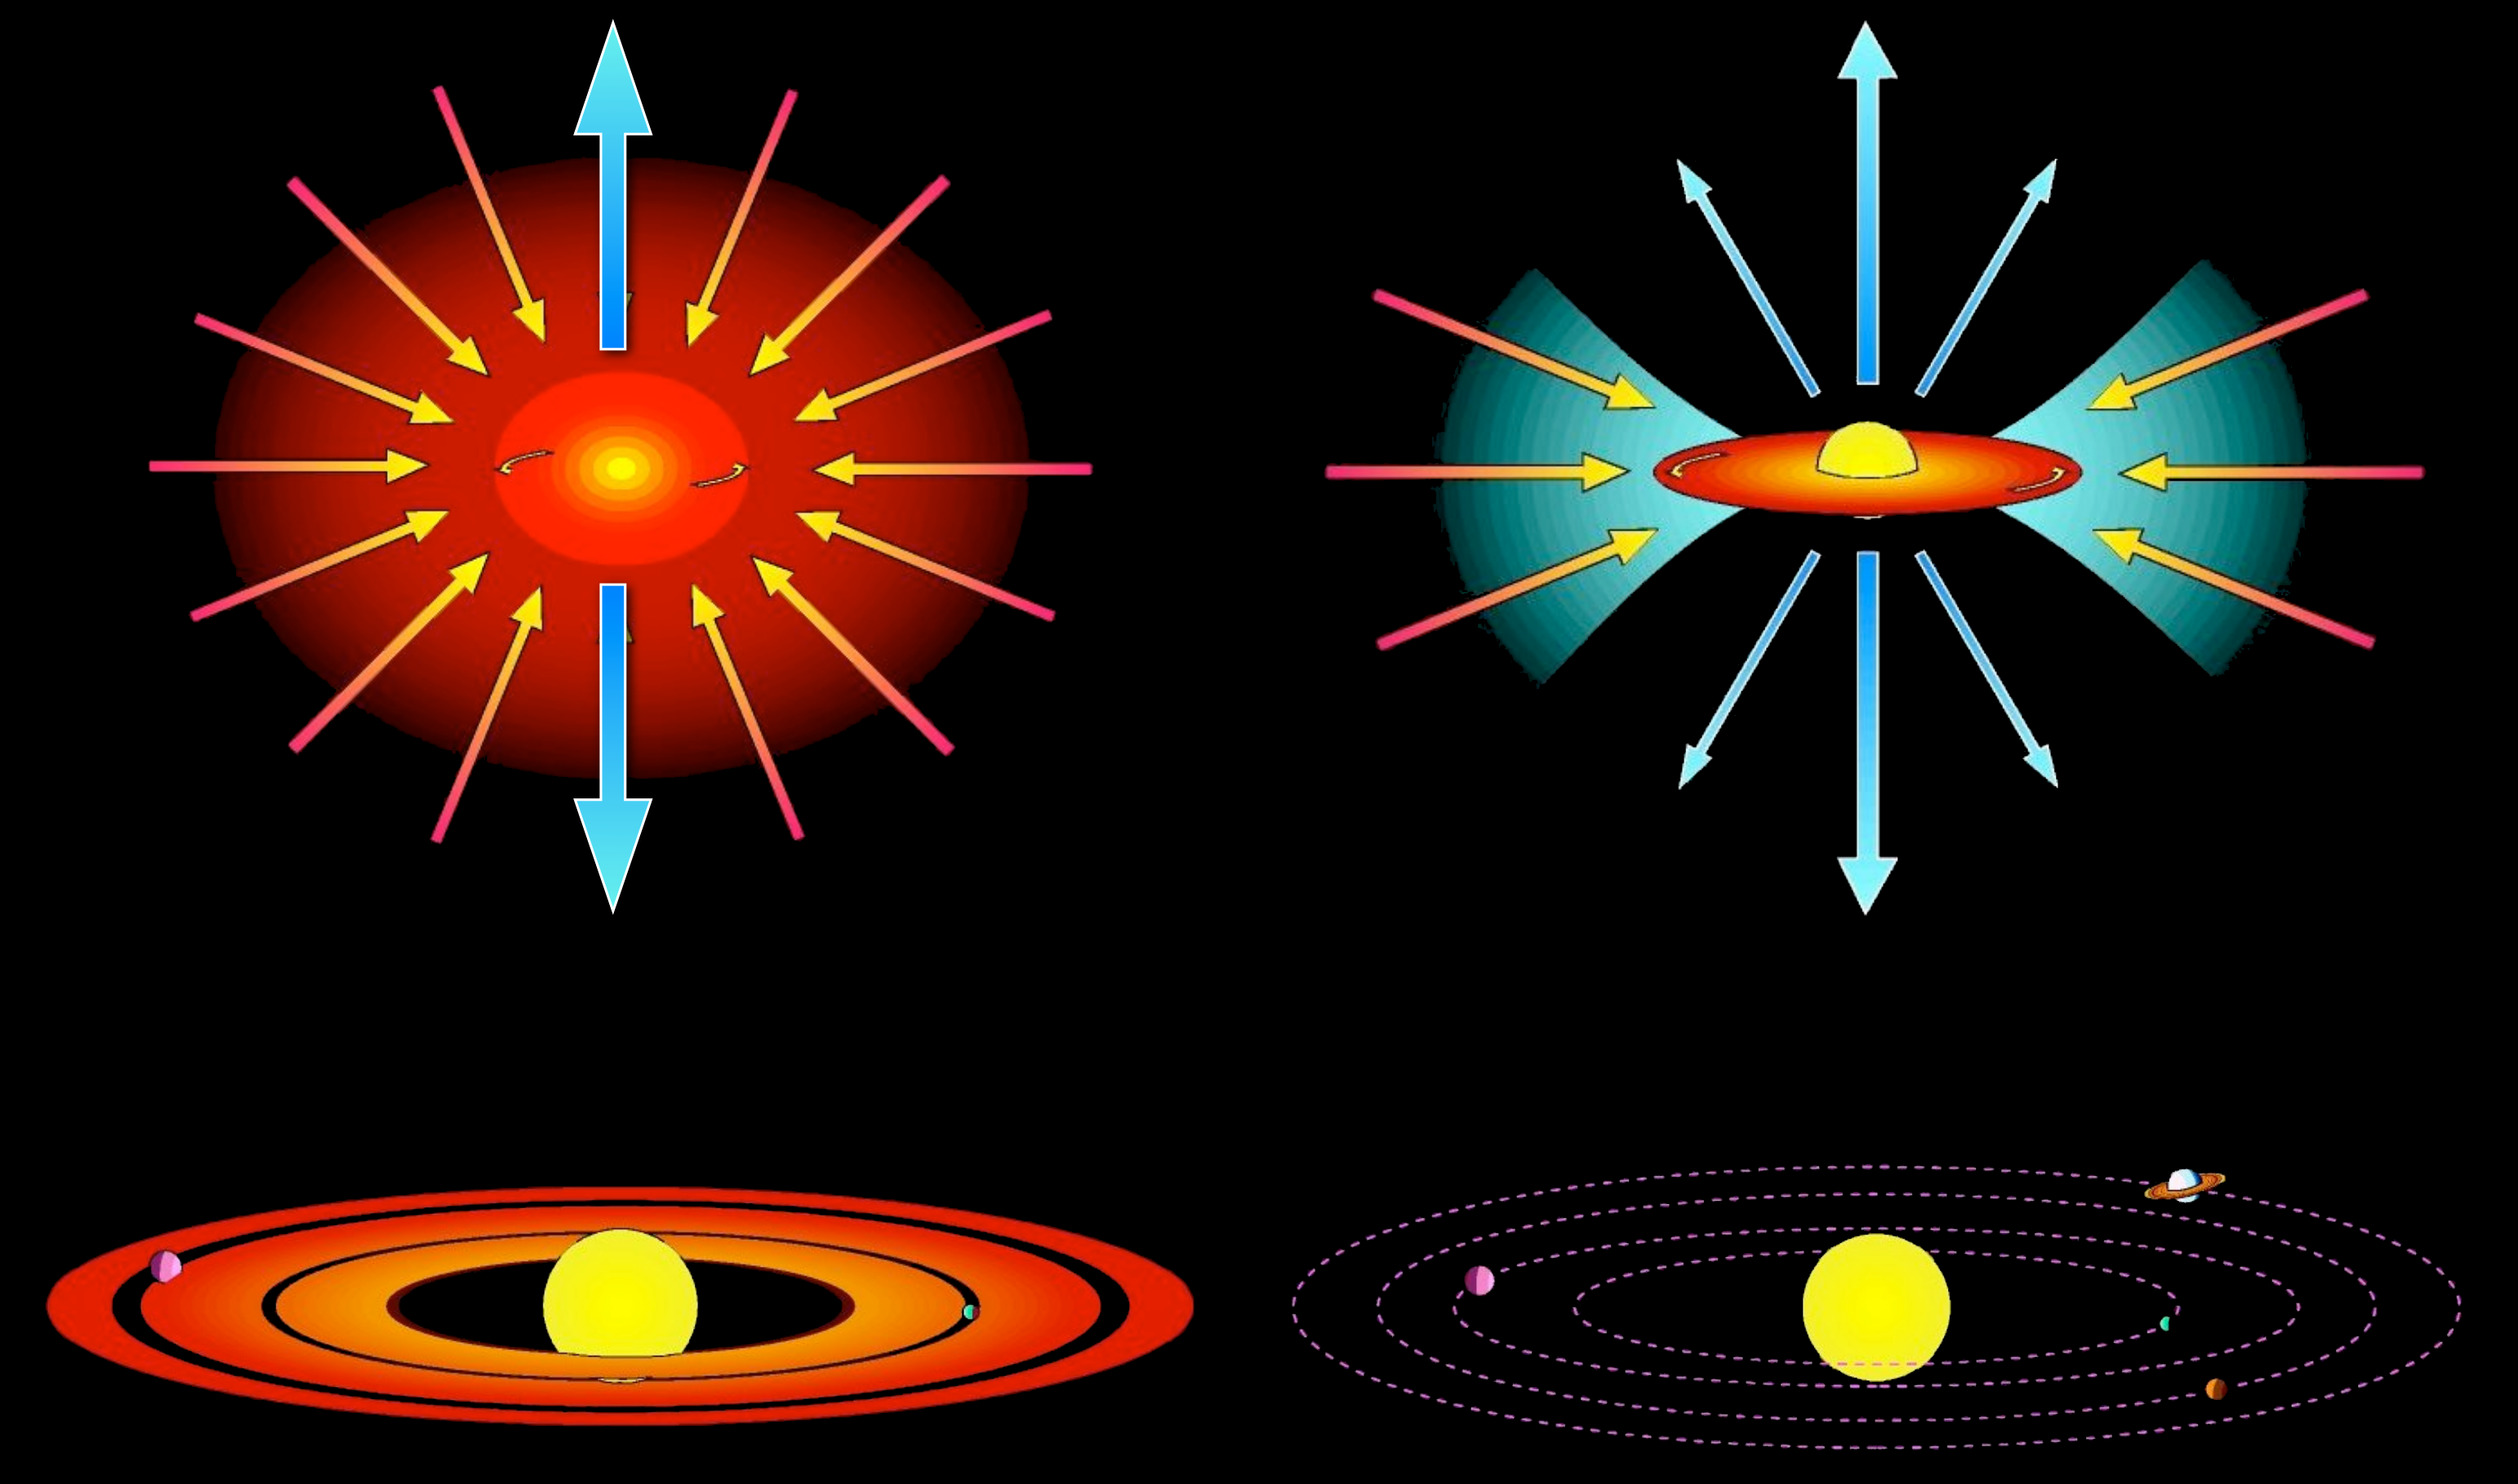
\includegraphics[width=10cm]{figs/starform_classes.png}
\caption{Star formation sequence. At first, the collapse is mostly radial (top left) until the conservation of angular momentum leads to the formation of a circumstellar disk (top right). Outflows carry away angular momentum (top row). Once the envelope disperses (between the top right and bottom left stage), the mass in the disk decreases, setting the time scale for planet formation (bottom left). Eventually, only mass in the central star or the planetary system remains (bottom right). (Adapted from original diagram by M.~McCaughrean. \label{fig:starform_classes}}
\end{figure}

Finally, the disk fully disperses and leaves behind a pre-main sequence star, perhaps surrounded by planetary system. The central star continues to contract until it reaches the main-sequence (MS, Fig.~\ref{fig:starform_classes} bottom right). Solar mass stars reach the MS after approximately 100\,Myrs, and they reside on the MS for over 10\,Gyr.

Within this sequence of star formation, the class~II objects (CTTS) stand out, because we can see the central objects relatively unobscured and gain a detailed picture of the physical processes, including planet formation, using a large variety of observational techniques including X-ray data. However, the physical processes, in particular accretion and outflows, are thought to remain largely unchanged throughout this sequence so that we can benefit from the unobscured view during the CTTS-phase to study them.

\subsection{T Tauri Stars}
T~Tauri stars were first described as a distinct class of objects  by \citeauthor{Joy_1945} in 1945 based on their pronounced optical variability \citep{Joy_1945}. The notion that T~Tauri stars are young came with the realization that they are located to the top right of  MS stars in the Hertzsprung-Russel diagram, consistent with the expected position of stars contracting along their Hayashi tracks towards the MS \citep{Hayashi_1961}. Also, strong Li absorption lines suggest a young age, because Li is quickly depleted in stellar photospheres, i.e., high photospheric Li abundances imply that there was not enough time to process the Li accreted from the molecular cloud \citep{Magazzu_1992}.
%
%
\begin{figure}[t]
\centering
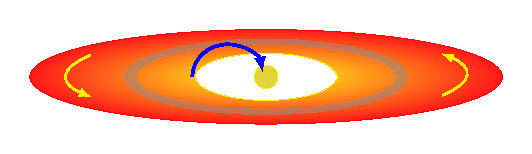
\includegraphics[width=10cm]{sketches/ctts.pdf}
\caption{Sketch of a classical T~Tauri system with an accretion disk and a wide-angle outflow. X-rays are coming from the stellar corona, the accretion shock and various points in the outflow. \label{fig:ctts_sketch}}
\end{figure}
%
On the other hand, the origin of other features like the strong emission lines like H$\alpha$, collectively termed “chromospheric emission”, remained controversial for a long time. The discovery of the infrared excess during the 1980s and the realization that CTTS are surrounded by cold dusty disks meant that disk accretion became a leading theory explaining many features, which is supported by the discovery that the ``chromospheric'' line profiles change from inverse to normal P~Cygni profiles and back within few days on individual systems. It is now well accepted that accretion 
and outflows are characteristic features of CTTS \cite{Bertout_2007}, in addition to their protoplanetary disks.

Disks, accretion, and outflows are the processes that define the properties of CTTS. Figure~\ref{fig:ctts_sketch} shows a sketch of a T Tauri system with the sources of the X-ray emission discussed in this chapter marked.
During the CTTS phase, the stellar mass is already close to the final value but the interior of the star is still fully convective \citep{Stahler_2004}, which together with rather rapid rotation (few days) leads to a strong stellar dynamo. Stellar magnetic fields during the CTTS phase are therefore in the kG range \cite{2008MNRAS.386.1234D,2010MNRAS.402.1426D}. Such strong magnetic fields disrupt the disk within a few stellar radii, because the hydrostatic star rotates slower than an approximately Keplerian disk. The interaction of the stellar magnetic field with the inner parts of the disk slows the innermost disk material down so that it cannot resist gravity and is channeled along the stellar magnetic field lines onto the star. It is accelerated to almost free-fall velocity and impacts the stellar photosphere where a strong shock forms. The details of the accretion shock are described in the next section.

The inner disk would be depleted within $10^3$ to $10^4$ years without being replenished by material from outer disk radii. Therefore, continued accretion requires radial transport of material through the disk which in turn requires the redistribution of angular momentum (AM). Several processes have been invoked to promote this AM redistribution. Prominent examples include the magneto-rotational instability \citep[MRI,][]{Balbus_1991} with non-ideal magnetohydrodynamic (MHD) extensions and disk winds \citep{Blandford_1982, Pudritz_1983}. In reality, the vertical structure of protoplanetary disks likely results in different transport mechanisms dominating at different disk heights with most of the mass being transported through the upper disk layers where magneto-centrifugally driven winds are launched.

Those winds require some net vertical magnetic field threading the disk. Material is accelerated along magnetic field lines until the magnetic field strength becomes insufficient to control the particle motion and the Lorentz force causes the collimation of the outflowing material into narrow jets. The jet velocity depends on the so-called magnetic lever arm, which relates the (approximately) Keplerian velocity at the launch radius to the jet velocity and is of order 10 \citep{Ferreira_2006}; hence, jet velocities are on the order of 300\,km\,s$^{-1}$. In addition to disk winds, there may be other outflows like stellar winds, magnetospheric ejections (from the star or the star-disk interaction region), or the so-called X-winds from the inner disk edge \citep{Shu_1994}.

At some point, typically after a few Myrs, the disk has dispersed \citep{2009AIPC.1158....3M} and we are left with a pre-main sequence star, possibly with a number of orbiting planets. Such objects are called weak-line T~Tauri stars (WTTSs), which show no signatures of neither accretion nor outflow activity.

\subsection{The power of X-rays for studying T~Tauri stars}
The different parts of a classical T~Tauri system have grossly different temperatures: The disk midplane may be characterized by only few 10~K, the upper disk layers are likely above 1000~K, the inner edge of the disk is typically assumed to be around 2\,000~K, and stellar photospheric temperatures are 3-4\,000~K for CTTS. Therefore, the intrinsic emission of these different components peaks in very different wavebands, which is reflected in the observational tools used to study them. Sub-mm radio to IR observations enjoy great popularity for disk studies while optical to NIR data are powerful for studying the more dynamic processes such as accretion and outflows. There are, however, some interesting exceptions, e.g., FUV data probe the hydrogen content of the inner disk as well as accretion \citep[see review in][]{Schneider_2020}.

On first sight, it may therefore appear surprising that X-ray observations play an important role for studying CTTS. However, a flow with velocities in excess of 300\,km\,s$^{-1}$, which rams into a stationary obstacle shock heats the post shock plasma to temperatures in excess of 1\,MK. The radiation from such a plasma peaks in the X-ray regime and the shock-powered X-rays directly probe the shock region and not ``just'' reprocessed emission as seen in other wavelengths. Thus,  X-ray studies of accreting objects are powerful diagnostics for in- and outflow processes. 
